\section{Evaluation}
During the course of the project, feedback was repeatedly sought from clinical staff in regards to the progression of SANSURGIMS. This feedback was not only valuable to the student in regards to designing but also necessary in order to ensure continued alignment with requirements and staff needs. Towards the end of the project, this staff feedback was complimented with a questionnaire in order to attain quantifiable values that would lend themselves analysis. The student's view of SANSURGIMS was not included in any evaluation because end-users make much better judges when used in conjunction with measurement instruments as they, the end-users, tend to see things more in regards to strategic benefits for the organisation as opposed to the more system-benefit centric view of an IS professional (\cite{MiraniLederer}). This leads to an overarching statement of IS Success and is said best by \cite{Seddon}:

\begin{quote}
\center\emph{``IS Success is [...] conceptualized as a value judgement made by an individual, from the point of some stakeholder."}
\end{quote}
\vspace{6mm} 
 
\subsection{Testing Procedures}
As mentioned above, the evaluation of the system was undertaken in two forms. The first form of evaluation, direct user feedback, was utilised during the majority of the project lifespan. The student met with clinical staff repeatedly and presented them with the current system. The student was accompanied by another student during these feedback sessions that was responsible for assisting in taking notes. This way, the student was able to give the clinical staff his full attention and facilitate a constructive session. 
\\ \\
The second form of evaluation undertaken was the use of a questionnaire at the end of the project (Appendix \ref{Clinical Handover Questionnaire}). The questionnaire first asked the clinical staff member to navigate to the handover for a specific patient and then answer specific questions about that patient. The task was used to determine how well the user could navigate the system and if he or she could find information in an acceptable time frame. After completing the small tasks, the clinical staff usually gave feedback in regards to the handover form on their own accord. After their feedback was noted, the clinical staff member was asked to answer the questions on the questionnaire. The objective of the questionnaire was to present the staff member with a small number of questions to which the he or she only needed to circle the statement that most corresponded with their view. It was very important that the questionnaire be short and easy to fill out in order to not give the clinical staff the feeling that reviewing the system was a very time consuming matter. This plays an important role in regards to obtaining subsequent feedback. If staff feel that reviewing the system is too time consuming they might refrain from giving feedback.

\subsection{Test Results}

The continual feedback received from various clinical staff included a range of responses. These ranged from being very positive about the work being done to citing short comings of SANSURGIMS or even misconceptions introduced by the student. The feedback was always perceived as constructive and the student believes that these responses were earnest views of the system. 
\\ \\
In regards to the questionnaire, the responses were mostly positive. There were some issues with navigating the system where clinical staff did not see the handover button on the right side of the table and instead opted to click on the row within the table. Others were uncertain when using the system and paused for one to two seconds before clicking the button. A third group of users were more confident in using the system and did not hesitate. The questions in the tasks were answered in a timely matter for the most part with only one user needed considerable longer to find the information. This stemmed from the fact that the user was taking longer to orientate themselves within the system than other users. The average rating in the questionnaire by question is displayed below:

\begin{figure}[hp]
				\centering
				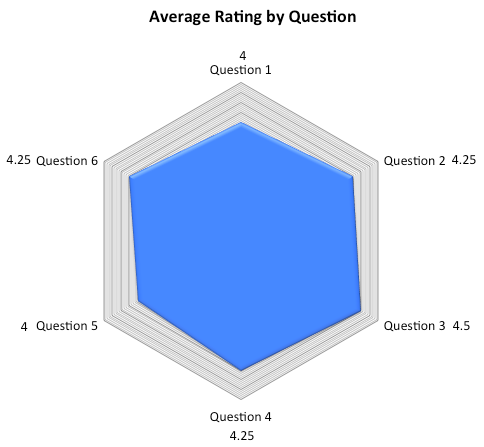
\includegraphics[scale=1.0, width=80mm]{Images/Evaluation-Results}
				\caption{Questions Results - Averaged}
\end{figure}

\newpage
\subsection{Interpretation of Results}
While staff feedback was viewed as earnest and constructive in regards to SANSURGIMS, it nevertheless needs to be taken with a grain of salt. This stems from the fact that there are numerous influences acting on a stakeholder and each will affect how the stakeholder views and acts during the project. In regards to the clinical staff, one could argue that time pressures and the fact that they were not consulted on whether to have such a project be undertaken on their ward or not lead to a lack of full support. The staff was very helpful but the amount of support might have been greater had 
mention that you only had 4 users for the questionnaire

